\section{AI-Agents in General (RQ2)}
\label{sec:ai-agents}
zunächste soll geklrät werden was unter KI-Agenten verstanden wird.
Letztlich sind KI-Agenten system um teilaufgaben zu automaiseren.
Um eine präzieres Verständnis zu bekommen lohtn es sich daher eine abgrezung zu klasssen worklof
automatiserungen zu machen.

Programmatische Prozessautomatisierung bezeichnet die regelbasierte Automatisierung von Abläufen, bei der
festgelegte Bedingungen und strukturierte Entscheidungslogiken genutzt werden, um Prozesse effizient,
zuverlässig und wiederholbar auszuführen. Technicken die hier zum einsatz kommen sind robotic Process
Automation, Skritping und Markos.

LLMs können kontext ldabei helfen unstruktierte aufgaben zu lösen. antrhopic whält folgende Defintion bz von
Agenten welche KI-Agneten von Workflos abgrenzt.
Workflows are systems where LLMs and tools are orchestrated through predefined code paths.
Agents, on the other hand, are systems where LLMs dynamically direct their own processes and tool usage,
maintaining control over how they accomplish tasks.

% ---------------------------------------------------------------------------------------------------------------------
\subsection{Prompt Engineering and Context Engineering}
\label{sec:context-engineering}

Allgemein bezeichte Context engineering das Designen, organiseren und managen von kontexsenstiiver infromatioen,
so das machienen im einklaing mit der menschlichen intention aggieren. \cite[p. 3]{huaContextEngineering202025}

Obwohl das Context Engineering bereits in frühen Frameworks der Mensch-Computer-Interaktion eine Rolle
spielte \cite[p. 1]{huaContextEngineering202025}, hat die Forschung aufgrund der wachsenden Herausforderungen in der
Human-Agent-Interaction (HAI) in jüngster Zeit eine verstärkte Fokussierung auf dieses Gebiet erfahren.

Die Relevanz dafür sit begründet auf aktuellen Limitiationen (TODO Beispile), Performance Verbeserungen (TODO
Beispiele) und Resroucen Optmierung.

Mei et al. (2025) haben in ihrer Meta-Studi \cite{meiSurveyContextEngineering2025} über 1.400
Forschungsarbeiten zum Thema Context Engineering für LLMs analysiert.
Laut den Autoren haben sich LLMs von einfachen Systemen, die lediglich Anweisungen
befolgen (sog. Prompt Engineering), zu zentralen Schlussfolgerungsmodulen entwickelt. Dabei habe sich
die Gestaltung und Verwaltung von Informationsinhalten zu einer eigenständigen Disziplin weiterentwickelt
(Context Engineering) \cite{meiSurveyContextEngineering2025}

Bei agentenbasierter Systeme lässt sich Context Engineering wie folgt definieren:

\begin{quote}
  "Context engineering is the practice of deliberately structuring and optimizing the information passed to an
  LLM or Agent to produce more accurate and relevant outputs." \cite[00:34]{ibmtechnologyWhatContextEngineering2026}
\end{quote}

Damit geht Context Engineering über das klassische Prompt Engineering hinaus und umfasst erweiterte Methoden wie
Retrieval-Augmented Generation (RAG), Speichersysteme, Tool-integriertes Reasoning sowie Multi-Agent-Systeme
(vgl. Mei et al., 2025). \cite[p. 12-26]{meiSurveyContextEngineering2025}

Obwohl in der Literatur verschiedene Methoden zum Kontext Engineering diskutiert werden, weisen Mei et al.
kritisch darauf hin, dass die Praxis derzeit ohne einheitliche theoretische Grundlagen operiert. Diese
Grundlagen wären notwendig, um die unterschiedlichen Techniken miteinander zu verknüpfen und
prinzipienbasierte Entwurfsrichtlinien abzuleiten. Die Forschungslücke wird zudem durch das Fehlen
mathematischer Rahmenwerke verstärkt, die es ermöglichen würden, optimale Entwurfsprinzipien für das Kontext
Engineering in komplexen Systemen zu charakterisieren. Dies steht im Zusammenhang mit dem Mangel an Methoden
zur Bestimmung der optimalen Kontextzusammensetzung. \cite[p. 51]{meiSurveyContextEngineering2025}

%%%%%%%
% ---------------------------------------------------------------------------------------------------------------------
\subsection{Building blocks for AI-Agents}
\label{sec:ai-agent-building-blocks}

Um den späteren AI-Agent zu bauen, war es notwenidg sich zunächst mit den Grundbausteinen der KI-Agenten zu
beschäftigen. Antrhopic hat dies bezüglich eine Blogpost veröffetnlicht welcher die Grundbauseite aus deren
Sich zusammenfasst \cite{anthropicBuildingEffectiveAI}.

\textbf{Prompt chaining}

\begin{figure}[htbp]
  \centering
  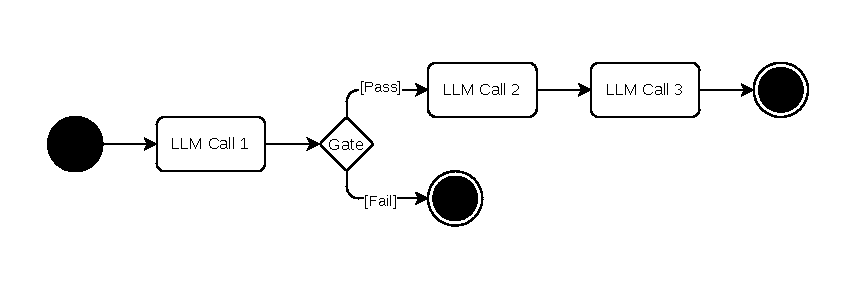
\includegraphics[width=0.9\textwidth]{assets/figures/prompt-chaining.pdf}
  \caption{Prompt chaining: A complex task is decomposed into sequential LLM calls
    \figsource{Own illustration based on "Building Effective AI Agents by
  Anthropic"\cite{anthropicBuildingEffectiveAI}, created with draw.io.}}
  \label{fig:prompt-chaining}
\end{figure}

In prompt chaining, a complex task is broken down into a sequential series of substeps. Each step is
described by a prompt and an LLM call, which uses the result of the previous step as context for the next step.
Programmatic checks can be inserted in between.

\textbf{Routing}

\textbf{Parallelization}

\textbf{Orchestrator-workers}

\textbf{Evaluator-optimizer}

\textbf{Augmented LLM}

Diese Workflows orientieren sich an klaren Argumentationsketten. Die Informationen folgen einem im Code
prozedural gesteuerten sequenzeller Weg, während LLM-Aufrufe bewusst für entsprechende Teilaufgaben mit einer zuvor
bekannten Intention stattfinden. Mit anderen Worten: Es existieren vordefinierte, klare Pfade, denen die
Daten sowie die Ausgaben der LLM-Aufrufe folgen.

Bei Agenten gibt es diese kar vordefinierten prozeduralen Pfade in dem sinne nicht. Das LLM
selbst wird genutzt, um zu entscheiden, welche Wege eingeschlagen werden sollen.
Dies kann insbesondere bei offenen Problemen hilfreich sein, die sich nicht ohne Weiteres in einem starren
Workflow abbilden lassen.
Dabei wird das LLM mit verschiedenen Tools ausgestattet, und es bleibt dem Modell überlassen, ob und wann es diese Tools
aufruft. Die Qualität des Gesamtoutputs hängt somit auch davon ab, wie zuverlässig das LLM das korrekte Tool
auswählt. Dies abstrahiert offene Probleme in eine Struktur, in der Tool-Calling in einer Schleife
stattfindet, bis das LLM selbst entscheidet, dass das gewünschte Ergebnis erreicht ist.

%%%%%
Diese workflows orienteirren sich an klaren Argumentationsketten. Die Infroamtionen folgen einem im code
procedural gesteuretem weg und llm calls finden intentila für entsprechende unteraufgaben mmit einer vorher
bekannt intention zu einem squenziall beaknten zeitrahmen statt. Anders ausgerdück gibt es vordefinierte
klare Wege, welche die Daten und die outputs der LLM-Calls folgen.

Folgt man der Definition von Athropic werden diese klaren vordefinierten entfernt und ein LLM wird
genutzt um selbst zu entscheiden, welche wege eingeschalagen werden. Dies kann besonders offene Problme
hilfreich sein, die nicht einfach in einem Workflow eingefangen werden können. Hierbei wird ein LLM mit
verscheinde Tools ausgestattet und es dem llm wird überlassen ob es dieses Tool aufrufen wird. Die Qualtiät
des gesamt outputs häng somti auch damit zusammen wie zuverlässig dass LLM das korrekte Tool aufruft. Dies
abstrahiert somit offene Problme in eine struktur in der Tool-Calling in a Loop stattfinde, bis das LLM
selbst entscheiden, wann das gewünsche ergbeniss erreicht ist.

Wrokflos Desing lassen smoit granularer Kontroole zu, während Agents etwas losgelöster aggieren können.

% ---------------------------------------------------------------------------------------------------------------------
\subsection{Evaluating and Testing of AI-Systems}